\documentclass[a4paper,11pt]{scrreprt}
    %% Used for changing geometry of the page
    %% Cover page text cannot overlay cover sketching/style
    %% https://ctan.org/pkg/geometry?lang=en
\usepackage{geometry}
    %% Changes language of some packages protocols
    %% e.g., when captioning images: Figure 1. -> Figura 1.
    %% https://ctan.org/pkg/babel?lang=en
\usepackage[portuguese]{babel}
    %% Used for special fonts
    %% Cannot be compiled with pdflatex
    %% https://ctan.org/pkg/fontspec?lang=en
\usepackage{fontspec}
    %% Arial FONT
    \setmainfont{Arial}
    %% More colors and color options
    %% https://ctan.org/pkg/xcolor?lang=en
    %% https://ctan.org/pkg/colortbl?lang=en
\usepackage{xcolor,colortbl}
    %% More tabular options, like dashed/dotted lines
    %% https://ctan.org/pkg/arydshln?lang=en
\usepackage{arydshln}
    %% List of acronyms
    %% https://ctan.org/pkg/nomencl?lang=en
\usepackage[intoc]{nomencl}
    %% Must be called to init nomencl environment
    \makenomenclature
    %% More images options/settings
    %% https://ctan.org/pkg/graphicx?lang=en
\usepackage{graphics}
    %% Defining subdirectories to image path enviornment
    %% \graphicspath{{sub1}{sub2}...{subN}}
    \graphicspath{{images}}

    %% used to handle cross-referencing commands in LaTeX to produce hypertext links in the document
    %% https://ctan.org/pkg/hyperref?lang=en
\usepackage{hyperref}
    %% math environments
    %% https://ctan.org/pkg/amsmath?lang=en
    %% settings
    \hypersetup{
        colorlinks,
        citecolor=black,
        filecolor=black,
        linkcolor=black,
        urlcolor=black
    }

\usepackage{amsmath}
    %% Defining backgrouns, used to make the cover
    %% https://ctan.org/pkg/background?lang=en
\usepackage[some]{background}
    %% Used to make drawings or complex graphics
    %% http://pgf.sourceforge.net/pgf_CVS.pdf
\usepackage{tikz}
    %% Tikz library to point operations ((x1,y1) + (x2,y2))
    \usetikzlibrary{calc}

%% code snippets
\usepackage{listings}
\usepackage{color}

\definecolor{dkgreen}{rgb}{0,0.6,0}
\definecolor{gray}{rgb}{0.5,0.5,0.5}
\definecolor{mauve}{rgb}{0.58,0,0.82}

\lstset{
    frame=tb,
    language=C,
    aboveskip=3mm,
    belowskip=3mm,
    showstringspaces=false,
    columns=flexible,
    basicstyle={\small\ttfamily},
    numbers=left,
    numberstyle=\small\color{gray},
    keywordstyle=\color{blue},
    commentstyle=\color{dkgreen},
    stringstyle=\color{mauve},
    breaklines=true,
    breakatwhitespace=true,
    tabsize=3,
    moredelim=**[is][\color{blue}]{@}{@}
}

%% further RelaX definitions
%% \usepackage{stix}

%% Defining sfdefault font and default font for document
\renewcommand{\familydefault}{\sfdefault}

%% For tables
\usepackage{pbox}
\usepackage{longtable}
\usepackage{xcolor} % for coloring rows
\usepackage{multirow}
\usepackage{hhline}
\usepackage{array}

%==========================================================================
% DOCUMENT
%==========================================================================

\begin{document}

\pagenumbering{gobble}

%% Costume made cover
%% From there you can use \makecover command to build the cover
%% Blue cover color
\definecolor{titlepagecolor}{RGB}{60, 60, 60}

%==========================================================================
% COLORED BAR ON THE LEFT SIDE
%==========================================================================

\backgroundsetup{
    scale=1,
    angle=0,
    opacity=1,
    contents={
        \begin{tikzpicture}[remember picture,overlay]
            \path [fill=titlepagecolor] (-10.5,-15) rectangle ++ (5,30);
            \node[color=white] at (-7,-12) {\bfseries {\fontsize{120}{60} \textsf{S}}};
            \node[color=titlepagecolor] at (-4,-12) {\bfseries {\fontsize{120}{60} \textsf{O}}};
        \end{tikzpicture}
    }
}

%==========================================================================
% TITLE PAGE INFO
%==========================================================================

%% Changes values in this field to show information in the cover and back cover about your team/project

%% TITLE
\title{Orquestrador de Tarefas}

%% AUTHORS
\author{
    Flávia Alexandra Silva Araújo (A96587) \\
  \quad
    Miguel Torres Carvalho (A95485)
}

%% Date

\date{\today}

%% Course
\newcommand{\Course}{Licenciatura em Engenharia Informática}

%% Department
\newcommand{\Department}{Escola de Engenharia}

%% UniName
\newcommand{\UniName}{Universidade do Minho}

%% UniPic
\newcommand{\UniPic}{
\includegraphics[scale=0.09]{images/uminho.png}}

%% University
\newcommand{\University}{
    \begin{flushleft}
        \UniPic
    \end{flushleft}
    \textcolor{gray}{\small\textbf{\textsf{\UniName}}}\par
    \textcolor{gray!80!white}{\small{\textsf{\Department}}}\par
    \textcolor{gray!70!white}{\small{\textsf{\Course}}}
}

%% UC
\newcommand{\UC}{
    \begin{flushleft}
        \par\textcolor{titlepagecolor}{  \LARGE\textbf{\textsf{Unidade Curricular de \\ Sistemas Operativos}}}
    \end{flushleft}
}

%% School Year
\newcommand{\SchoolYear}{
    \small{\textsf{Ano Letivo de 2023/2024}}}


%% Define new command to show title, author and date
\makeatletter
\let\Title\@title
\let\Author\@author
\let\Date\@date
\makeatother

%% MAKETEMPLATE
\newcommand{\makecover}{

%% Removes page number on footer
\thispagestyle{empty}

%% No indentation
\setlength{\parindent}{0em}

%% Put Background defined on \backgroundsetup, in this page
\BgThispage

%% Changing geometry to prevent overlay with text
%% At the end of back cover, geometry is default with \restoregeometry
\newgeometry{top=5cm,left=6cm,right=3cm,bottom=2cm}

%% builds university info defined previously
\University
\vspace{1cm}
%% builds curricular unity info defined previously
\UC
%% builds school year info defined previously
\SchoolYear

\vspace*{5cm}
%% bigger space (i think its the default one) between paragraphs
\setlength{\parskip}{1em}

%% builds title info defined previously
\par\textbf{\textsf{\huge\Title}}
\vspace{1cm}
%% builds author(s) info defined previously
\par\Author

\vspace{0.5cm}

%% builds date info defined previously
\par\Date
\restoregeometry
\pagebreak

}


% builds the cover
\makecover

%% smaller footer and header size
\newgeometry{top=3cm,left=3cm,right=3cm,bottom=3cm}
\savegeometry{default}

%==========================================================================
% BEGIN OPCIONAL DEDICATÓRIA
%==========================================================================

% \clearpage
% \begin{center}
%     \thispagestyle{empty}
%     \vspace*{\fill}
%
%     $<<$/opcional Dedicatória$>>$
%
%     \vspace*{\fill}
% \end{center}
% \clearpage

%==========================================================================
% END OPCIONAL DEDICATÓRIA
%==========================================================================

%==========================================================================
% BEGIN ABSTRACT PAGE
%==========================================================================

%% Abstract name: \Large font size, flushed left and paragraph skip before abstract content
\renewenvironment{abstract}
 {\par\noindent\textbf{\Large\abstractname}\par\bigskip}
 {}

\begin{flushleft}
\begin{abstract}

    \textcolor{red}{>> Atualizar o resumo do relatório de acordo com as mudanças na segunda parte do trabalho.}

\end{abstract}
\end{flushleft}

\pagebreak

%==========================================================================
% END ABSTRACT PAGE
%==========================================================================

%==========================================================================
% BEGIN INDEXES PAGES
%==========================================================================

%% Changes table of content name
%% Portuguese babel default : “Conteúdo”
%% Personally I prefer “índice”
\renewcommand{\contentsname}{Índice}
\renewcommand{\listfigurename}{Índice de Figuras}
% \renewcommand{\listtablename}{Índice de Tabelas}

\tableofcontents

\pagebreak

\listoffigures

\pagebreak

% \listoftables
%
% \pagebreak

%==========================================================================
% END INDEXES PAGES
%==========================================================================

%==========================================================================
% BEGIN INTRODUCTION
%==========================================================================

%% Starting page numbering here
\pagenumbering{arabic}

\chapter{Arquitetura do Serviço}
    \section{Diagrama de Arquitetura do Serviço}
    \section{Descrição dos Módulos Desenvolvidos}
        \subsection{Orquestrador (\textit{orchestrator.c})}
        \subsection{Cliente (\textit{client.c})}
        \subsection{Pedido (\textit{request.c})}
        \subsection{Comando (\textit{command.c})}
        \subsection{Número de Tarefa (\textit{task\_nr.c})}
    \section{Diagramas de Comunicação entre Servidor e Cliente}
        \subsection{Execução e Agendamento de Tarefas}
            \newgeometry{top=3cm,left=0.1cm,right=0.1cm,bottom=4cm}
            \begin{figure}[!ht]
                \centering
                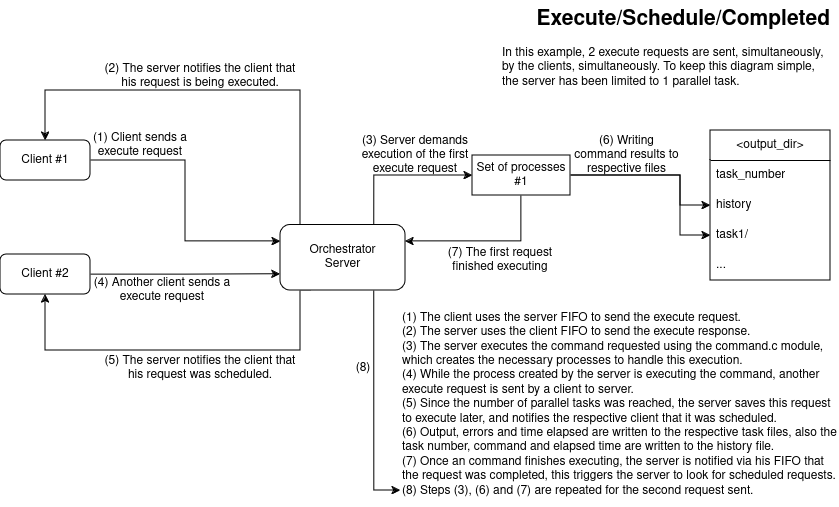
\includegraphics[scale=0.7]{diagrams/execute_schedule.png}
                \caption{Diagrama de Comunicação para Execução e Agendamento de Tarefas}
                \label{fig:3.1}
            \end{figure}
            \loadgeometry{default}
        \subsection{Estado de Tarefas}
            % \newgeometry{top=3cm,left=0.1cm,right=0.1cm,bottom=4cm}
            % \begin{figure}[!ht]
            %     \centering
            %     \includegraphics[scale=0.7]{diagrams/task_state.png}
            %     \caption{Diagrama de Comunicação para Estado de Tarefas}
            %     \label{fig:3.2}
            % \end{figure}
            % \loadgeometry{default}

\chapter{Argumentos da Interface de Linha de Comandos}
    \section{\textit{Orchestrator}}
    \section{\textit{Client}}

\chapter{Avaliação de Políticas de Escalonamento}
    No trabalho desenvolvido, foram implementadas três políticas de escalonamento de tarefas.
    Estas serão aprofundadas nas secções seguintes, assim como as suas avaliações práticas.
    Por favor consulte o anexo \nameref{anexo:2} para mais detalhes de como for realizada
    a implementação destas políticas.

    \textcolor{red}{>> Atualizar a introdução da avaliação de políticas de escalonamento.}
    \section{\textbf{FCFS} - \textit{First Come First Served}}
        Nesta política, as tarefas são executadas por ordem de chegada, o que não é
        eficiente em termos de tempo de espera e execução. No entanto, é uma política
        simples e fácil de implementar.

        \textcolor{red}{>> Escrever sobre a avaliação prática desta política + Imagem}
    \section{\textbf{SJF} - \textit{Shortest Job First}}
        A política \textit{Shortest Job First} é uma política de escalonamento não preemptiva
        que seleciona a tarefa com o menor tempo de execução, este tempo é passado como
        argumento na opção \textit{execute} do cliente e repesenta uma estimativa do tempo
        que a tarefa demorará a ser executada.

        Esta política é eficiente em termos de tempo de espera e execução, mas pode levar
        a situações de \textit{starvation}, que ocorrem quando tarefas com tempos de execução
        maiores são sempre adiadas, e num caso extremo, quando surgem constantemente tarefas
        com tempos de execução menores, estas de maior duração nunca serão executadas.

        Existem várias maneiras de lidar com situações de \textit{starvation}, como por exemplo
        a criação de uma especificação de tempo máximo de espera para cada tarefa, ou a
        definicação de um numero máximo de tarefas que podem ser executadas antes de uma
        tarefa com tempo de execução maior. Outra solução seria a implementação de uma
        política de escalonamento preemptiva, que permitiria a interrupção de tarefas em
        execução, para dar lugar a tarefas com tempos de execução menores.

        \textcolor{red}{>> Escrever sobre a avaliação prática desta política + Imagem}
    \section{\textbf{PES} - \textit{Priority Escalonation Scheduling}}
        De forma a evitar situações de \textit{starvation}, foi implementada a política
        \textit{Priority Escalonation Scheduling}. Nesta, as tarefas são executadas
        de acordo com a sua prioridade, que é definida pelo cliente na opção \textit{execute},
        simliarmente como o tempo estimado que é passado como argumento na política \textit{SJF}.

        As tarefas com maior prioridade são executadas primeiro, evitando
        situações de \textit{starvation}. As prioridades ficam a critério do cliente,
        possibilitando uma maior versatilidade na execução de tarefas, permitindo ao cliente
        definir a prioridade adequada para cada tarefa que deseja executar. No entanto, esta
        flexibilidade não garante a eficiência da execução das tarefas, caso estas não sejam
        corretamente priorizadas.

        \textcolor{red}{>> Escrever sobre a avaliação prática desta política + Imagem}

\chapter{Testes Desenvolvidos}

%==========================================================================
% BEGIN CONCLUSÕES
%==========================================================================

\chapter{Conclusões}
    \textcolor{red}{TODO escrever sobre interrupções do servidor e como este
    poderia lidar com estas}

    Após o desenvolvimento deste serviço, foram cumpridos todos
    os objetivos propostos no enunciado do trabalho, desde a implementação de
    uma interface de linha de comandos tanto para o servidor, como para o cliente,
    que permite a execução de tarefas do utilizador de forma assíncrona com a
    possibilidade de encadeamento de programas com \textit{pipes} e a
    consulta do estado das tarefas, assim como a implementação de um ficheiro
    \textit{log} para guardar as tarefas executadas e a implementação de um
    sistema com várias políticas de escalonamento e a avaliação prática destas.
    Também foi desenvolvido um conjunto de testes que permitem verificar o correto
    funcionamento do serviço.

    Após a afirmação da possibilidade da terminação ou interrupção do servidor
    pelo professor regente foi despertada a curiosidade de como o servidor
    poderia lidar com estas situações.

    Num estudo apronfundado desta unidade curricular, uma solução seria a
    implementação de um sistema de interrupções no servidor, que permitiria
    a este lidar com situações de terminação ou interrupção de forma mais
    eficiente, utlizando os sinais do sistema operativo para lidar com estas
    situações, evitando a perda de tarefas em execução e agendadas.

    Para tal, seria necessário lidar com tarefas em execução, guardando
    o estado destas em memória, e permitindo a sua correta terminação
    ou interrupção, assim como para as tarefas em espera. Estas poderiam
    ser guardadas numa fila de espera, que seria consultada sempre que
    uma tarefa terminasse, permitindo a execução da próxima tarefa na
    fila.

    Em suma, o desenvolvimento deste serviço permitiu a aplicação prática
    dos conhecimentos adquiridos ao longo do semestre, assim como a
    exploração de novas funcionalidades e conceitos, que permitiram
    a implementação de um serviço robusto e versátil, que permite a
    execução de tarefas de forma assíncrona, com a possibilidade de
    encadeamento de programas e a consulta do estado das tarefas.

%==========================================================================
% END CONCLUSÕES
%==========================================================================

%==========================================================================
% BEGIN BIBLIOGRAFIA
%==========================================================================

%% Changes biblibography name
%% Portuguese babel default : “Bibliografia”
%% Personally I prefer “Referências”
% \renewcommand\bibname{Referências}

%% https://www.overleaf.com/learn/latex/bibliography_management_with_bibtex

% %% Add bibliografia to index
% \addcontentsline{toc}{chapter}{Bibliografia}

%==========================================================================
% END BIBLIOGRAFIA
%==========================================================================

%==========================================================================
% BEGIN LISTA DE SIGLAS E ACRÓNIMOS
%==========================================================================

%% Portuguese babel does not translate this environment
% \renewcommand{\nomname}{Lista de Siglas e Acrónimos}

%% Text that can be shown before acronyms list
% \renewcommand{\nompreamble}{
%     \textcolor{red}{
%         <<Apresentar uma lista com todas as siglas e acrónimos utilizados durante a realização do trabalho. O formato base para esta lista deverá ser da forma como abaixo se apresenta.>>
%     }
% }

%% acronyms
% \nomenclature[01]{\textbf{SO}}{Sistemas Operativos}

%% Show acronyms
% \printnomenclature

%==========================================================================
% END LISTA DE SIGLAS E ACRÓNIMOS
%==========================================================================

%==========================================================================
% BEGIN ANEXOS
%==========================================================================
%
%% Why \addchap, instead of \chapter?
%% \addchap has no numbering but appears in table of contents.
\addchap{Anexos}

    \addsec{
        \href{anexos/refman.pdf}{\small \textcolor{blue}{[I] Documentação do Código Desenvolvido}}
        \label{anexo:1}
    }

    \addsec{
        \textcolor{blue}{
            \href{anexos/example.pdf}{\small \textcolor{blue}{[II] Implementação das Políticas de Escalonamento}}
        }
        \label{anexo:2}
    }

%==========================================================================
% END ANEXOS
%==========================================================================
\end{document}
